\documentclass[12pt,a4paper]{article}
\usepackage{graphicx}
\title{TurtleGraph 0.1 Spec}
\author{Anton Golov}
\begin{document}
	\maketitle{}
	\newpage
	\tableofcontents{}
	\newpage
	\section{Overview}
		TurtleGraph is a program that draws plots of functions.

		This spec is incomplete.  Please report any errors through the Issues system on github.

		\textbf{Note:} This spec has not yet been approved by the team.  Please review it and inform the author whether you have any suggestions/issues.

	\section{Scenarios}
		The following are a number of possible use-cases for TurtleGraph.  If you happen to know more, please add them to this document and inform the author.
		\subsection{Scenario: Alice}
			When doing her algebra homework, Alice occasionally needs to plot the function she is working with.  She turns on TurtleGraph and inputs the function she currently wants to see.

	\section{Goals}
		The goals for this version are:
		\begin{itemize}
			\item The interface should allow for the input of one function.
			\item The position of the axes and the scale must be configurable.
			\item Functions must be able to contain multiplication, division, addition, subtraction, exponentiation, parentheses, and one variable (x).
			\item After a graph is plotted, it should be possible to plot a second one on a clean canvas without restarting the program.
			\item At release time, there should be no open bug reports.\footnote{Work on 0.2 should not begin until 0.1 is released.}
		\end{itemize}

		A number of features are unrealistic to achieve for version 0.1.  These are labelled `non-goals', and the following are currently known:
		\begin{itemize}
			\item There is no need to allow for more than one graph.
			\item There is no need for functions that find the roots or top of the graph, or for calculating the area under it.
			\item The speed is not to be taken into account; optimisations should be discarded in favour of readibility.
		\end{itemize}

	\section{Interface}
		The interface should resemble \ref{fig:interface1}, and must at least provide that functionality.  It may also have a menubar, which would allow the user to quit the program, display an About dialogue, or display a help dialogue.
		\begin{figure}[h]
			\label{fig:interface1}
			\centering
			    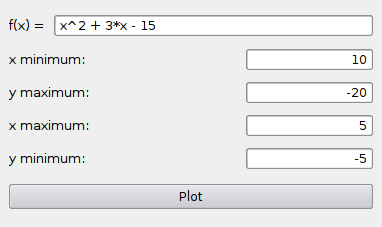
\includegraphics[width=\textwidth]{interface1.png}
			\caption{An approximation of the interface.}
		\end{figure}

\end{document}
